\section{System}

\subsection{WatchBox vs PlayList}
Mimicking the idea of internet radio, {\sys} abstracts the idea of
your current streaming queue as your playlist, and differentiates that
from the list of songs or shows you want to watch later, your
WatchBox.  In general, users will browse for shows they want to watch
and add these shows to their WatchBox.  Depending on what they feel
like watching at that moment, users will add shows from their WatchBox
to their playlist.  Once they watch the show from their playlist, it
is removed from their WatchBox.  The WatchBox playlist model means the
user ultimately has the power in deciding what they watch in the
moment.  They can remove things or add things from both their queue
and their watchbox.  If there are currently no shows in your playlist,
then {\sys} will recommend shows, either pulling the shows currently
in your WatchBox or using our situational recommendation system to
recommend a new show.  Users can override or remove any recommendation
at any time.

\begin{figure}
\centering
\subfloat[Browse for shows and add them to your WatchBox] 
{\label{fig:model1}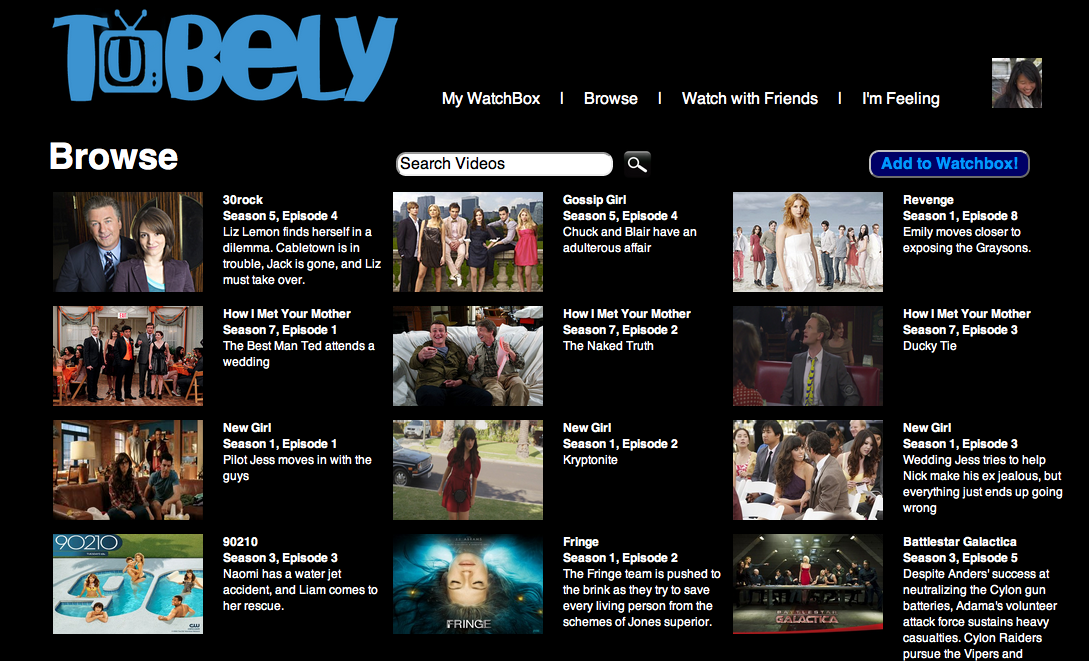
\includegraphics[width=0.24\textwidth]{pics/browse.png}}
~~\subfloat[Add shows from your WatchBox to your playlist] {\label{fig:model1}
\includegraphics[width=0.24\textwidth]{pics/watchbox.png}}
\caption{Browsing and adding shows to your WatchBox}
\label{fig:watchbox}
\end{figure}

\subsection{Watch with friends}
Most current social television apps want to help the user broadcast
what they’re watching and converse with others over chat about what
they’re watching.  {\sys} aims to address watching in real time and
encourage real life interaction.  {\sys} mainly does this by making
recommendations based on what friends you are hanging out with.
Normally, whenever people watch television with friends, they end up
flipping through channels, not knowing what to watch.  Alternatively,
too many people might want to watch different programs, resulting in
feuds over the remote.  {\sys} fixes these problems, recommending
shows based on the union of the group’s preferences.

Through Facebook, {\sys} will scrape all of a user’s friend list.  The
user will choose the friends they are with, and then {\sys} will
recommend three shows based on our situational recommendation model.
The user can either choose one of the three shows to start watching,
or press ‘Surprise me!’, which will automatically dump one of the
three shows into the currently streaming playlist.

Although {\sys} aims primarily at bringing people together in real
life, we understand that sometimes it is not always physically
possible.  Thus, we also support watching with friends virtually.
Similar to the current television viewing room model, users can join
in on friends who are already watching a show.

In general, {\sys} aims at bringing people together around the
television.  Instead of focusing on broadcasting what the user is
currently watching, {\sys} encourages users to watch tv with other
people.

\subsection{Mood}
Drawing from Pandora’s model, {\sys} allows the user to specify what
they’re in the mood to watch.  Viewers will select a mood based on
specialized categories that are found based on a detailed tagging
system.  There will be the typical genre selections, such as comedy,
drama, and reality.  However, this tagging system enables more
specific categories.  For instance, the ‘girly’ category may contain
shows like Gossip Girl or The Hills.  The ‘trashy’ category will have
shows like Jersey Shore or the Real Houswives.

\begin{figure}
\centering
\subfloat[Viewer chooses friends to watch with] {\label{fig:model1}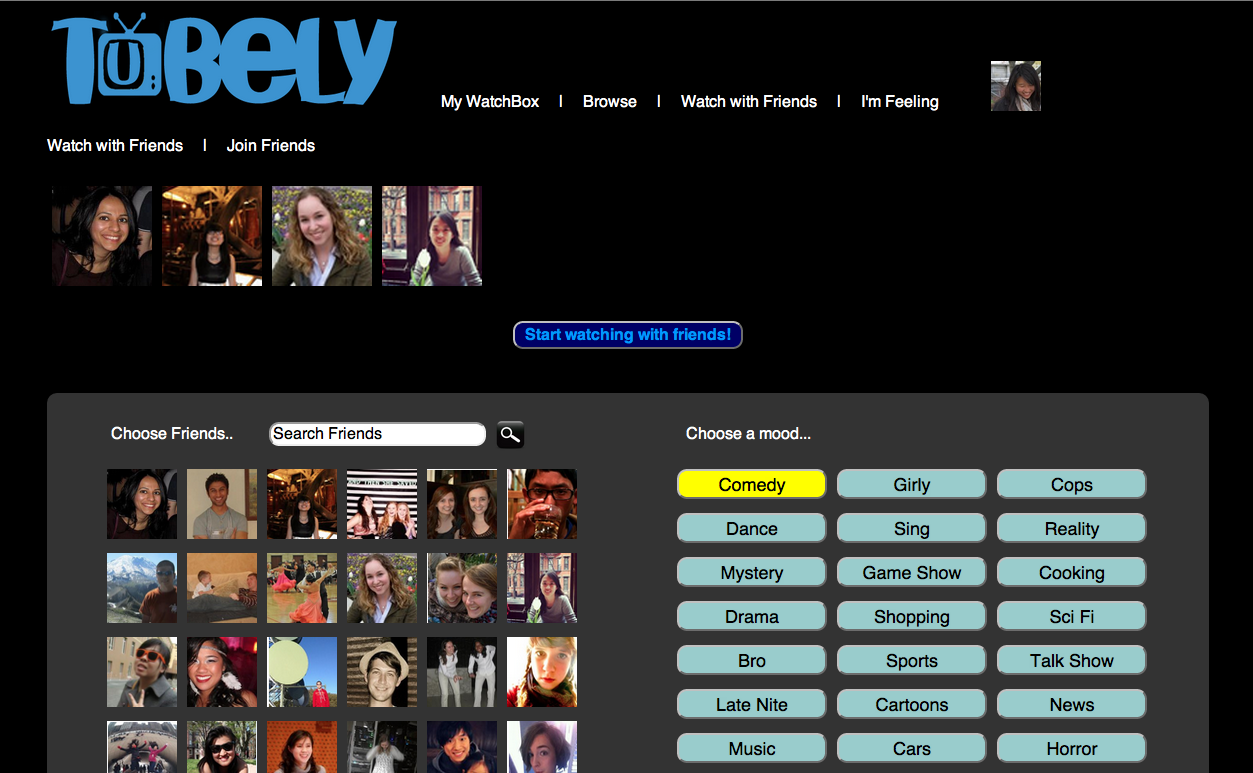
\includegraphics[width=0.24\textwidth]{pics/choosefriends.png}}
~~\subfloat[Viewer chooses from one of the three recommended shows] {\label{fig:model1}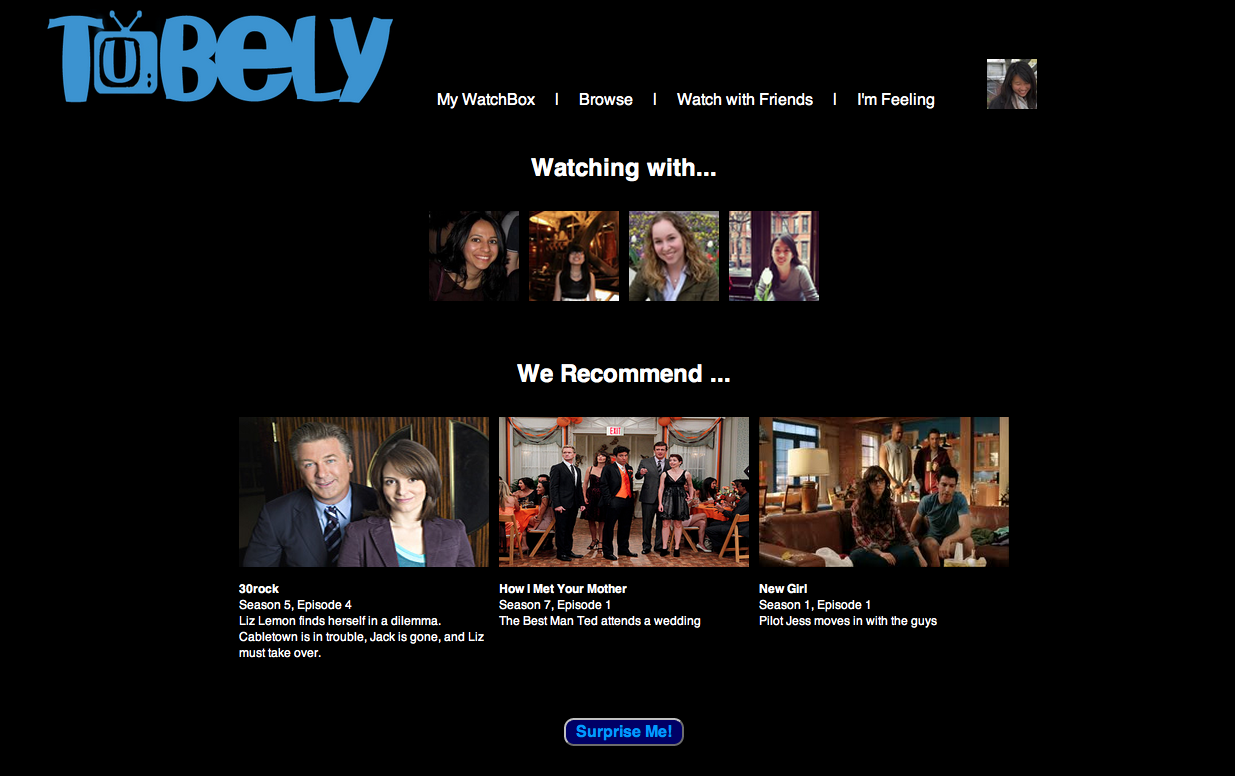
\includegraphics[width=0.24\textwidth]{pics/chooseshow.png}}
\caption{Watching with friends}
\label{fig:friends}
\end{figure}

A user may select multiple moods if they are watching alone, or if
they are watching with friends.  If they are alone, they will be
directed to the viewing area, and their playlist will be pre-populated
with shows that reflect the moods they chose.  The playlist will first
be populated with shows from your WatchBox that match the mood, and
then subsequently with recommended shows based on our recommendation
algorithm.  If the user is viewing with friends, we’ll recommend three
shows, taking into account both you and your friend’s preferences, as
well as what mood you’re in.

\begin{figure}
\centering
\subfloat[Viewer chooses from a mood] {\label{fig:model1}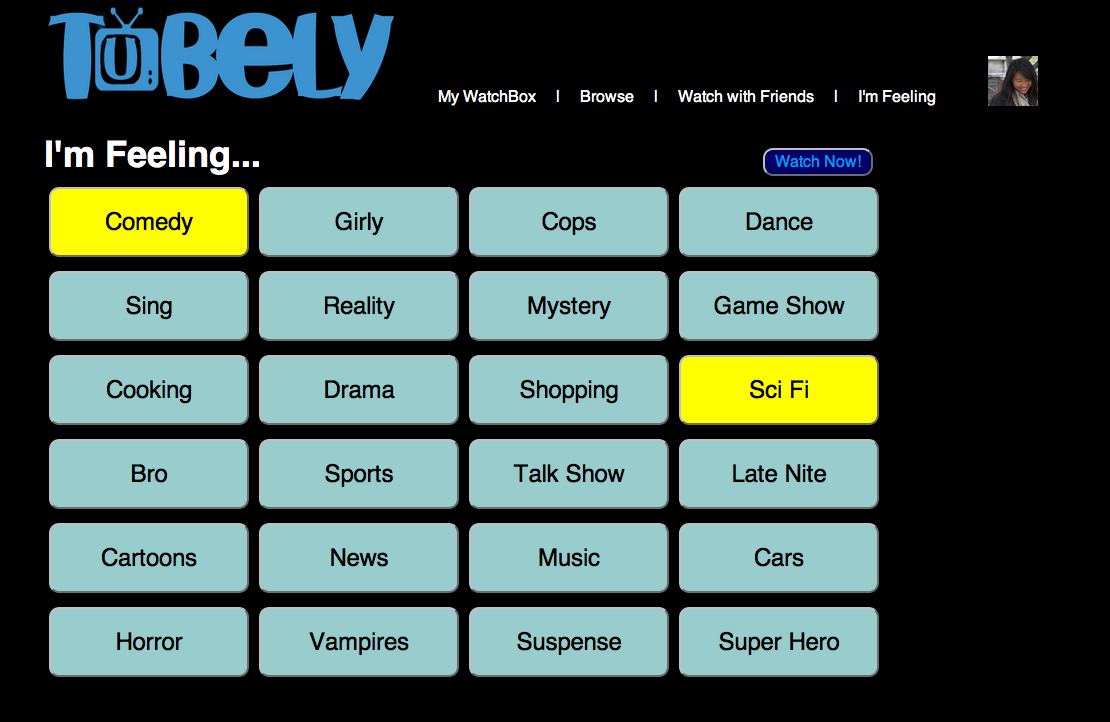
\includegraphics[width=0.24\textwidth]{pics/mood.png}}
~~\subfloat[Viewer chooses from a mood while watching with friends] {\label{fig:model1}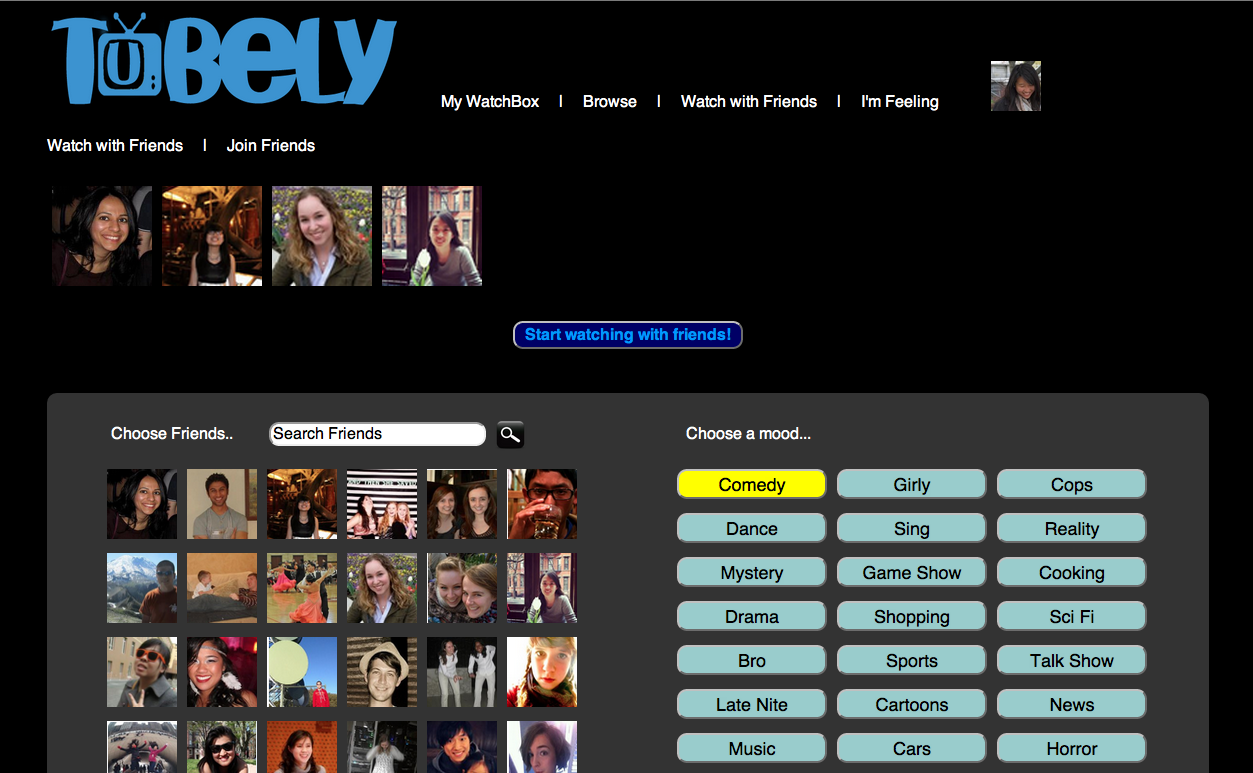
\includegraphics[width=0.24\textwidth]{pics/choosefriends.png}}
\caption{Choosing a Mood}
\label{fig:mood}
\end{figure}

\subsection{Implementation}
{\sys} runs on a Python Flask server and uses Jinja
templating~\cite{flask,jinja}.  It is coded in HTML/CSS/javascript and utilizes JWPlayer
for its embedded video player and playlist functionality~\cite{jwplayer}.
